\documentclass[border=5]{standalone}
\usepackage{tikz}
\begin{document}

\vbox {

\hbox{
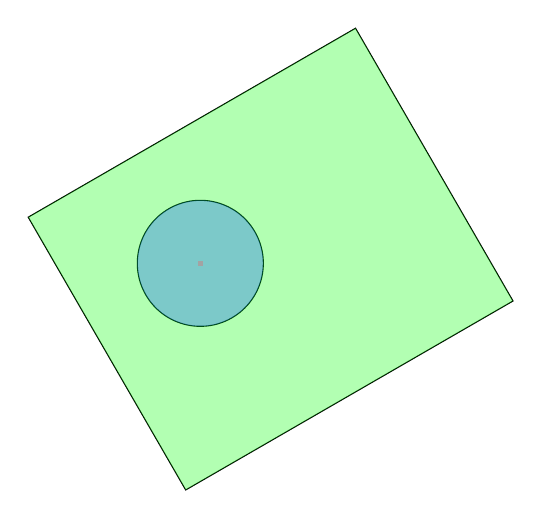
\begin{tikzpicture}[fill opacity=0.3, blend mode=screen, rotate=30, scale=0.8]
  \node[fill=red, inner sep=1pt] at (0, 0) {};
  \path[draw=black, fill=blue] (0,0) circle (1);
  \path[draw=black, fill=green] (-2,2) rectangle (4, -3);
\end{tikzpicture}

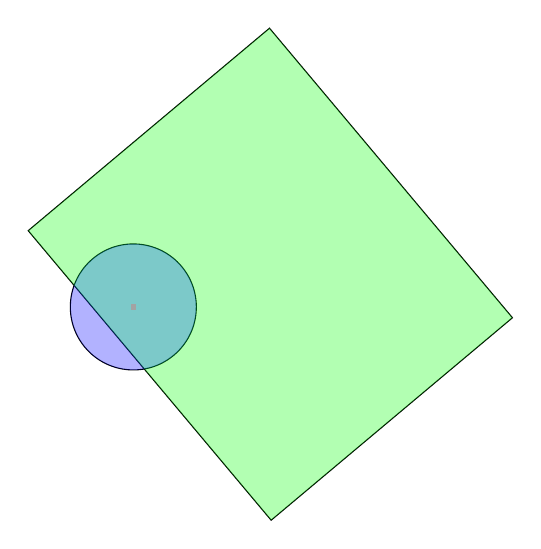
\begin{tikzpicture}[fill opacity=0.3, blend mode=screen, rotate=130, scale=0.8]
  \node[fill=red, inner sep=1pt] at (0, 0) {};
  \path[draw=black, fill=blue] (0,0) circle (1);
  \path[draw=black, fill=green] (-4,0.5) rectangle (2, -4.5);
\end{tikzpicture}

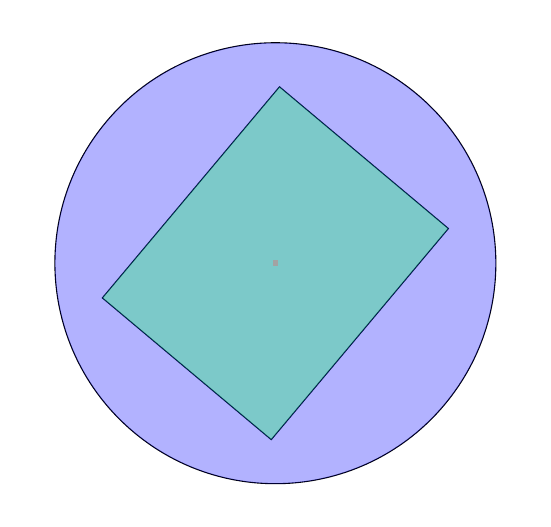
\begin{tikzpicture}[fill opacity=0.3, blend mode=screen, rotate=230, scale=0.7]
  \node[fill=red, inner sep=1pt] at (0, 0) {};
  \path[draw=black, fill=blue] (0,0) circle (4);
  \path[draw=black, fill=green] (-2.5,-2) rectangle (2.5, 2);
\end{tikzpicture}
}

\hbox{
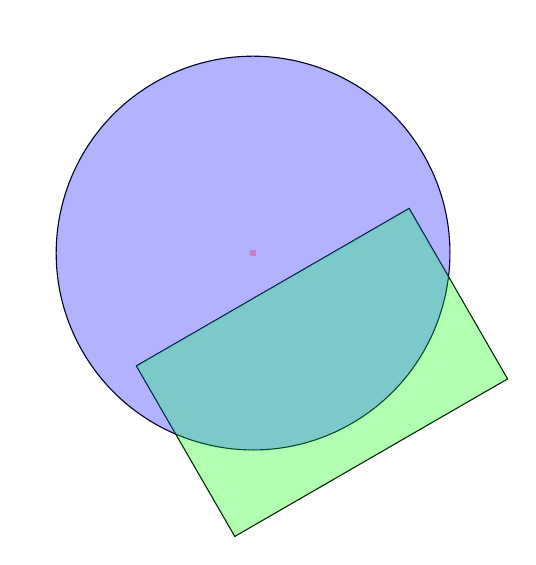
\begin{tikzpicture}[fill opacity=0.3, blend mode=screen, rotate=120]
  \node[fill=red, inner sep=1pt] at (0, 0) {};
  \path[draw=black, fill=blue] (0,0) circle (2.5);
  \path[draw=black, fill=green] (-3,-2) rectangle (-0.5, 2);
\end{tikzpicture}

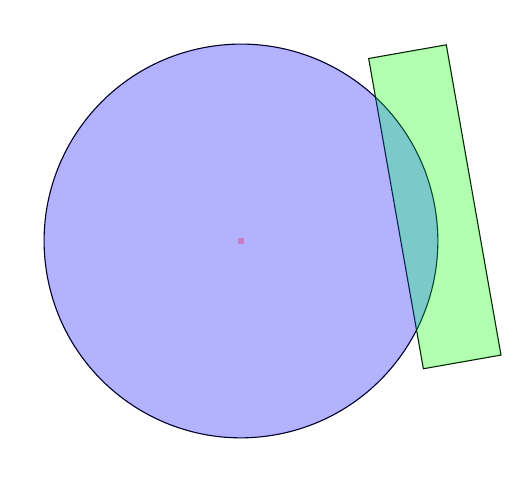
\begin{tikzpicture}[fill opacity=0.3, blend mode=screen, rotate=10]
  \node[fill=red, inner sep=1pt] at (0, 0) {};
  \path[draw=black, fill=blue] (0,0) circle (2.5);
  \path[draw=black, fill=green] (2,2) rectangle (3, -2);
\end{tikzpicture}

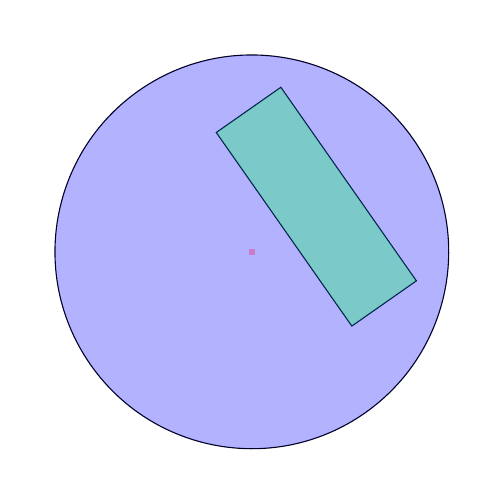
\begin{tikzpicture}[fill opacity=0.3, blend mode=screen, rotate=-55, scale=0.5]
  \node[fill=red, inner sep=1pt] at (0, 0) {};
  \path[draw=black, fill=blue] (0,0) circle (5);
  \path[draw=black, fill=green] (-3,1) rectangle (3, 3);
\end{tikzpicture}
}
}
\end{document}
